% ============================================================
% Manuscript prepared for Nature Machine Intelligence style review.
% Figures, tables, and numeric results are regenerated by:
%   cd submission/code
%   pip install .
%   uqqaoa-reproduce --output-dir . --depth 3 --budget 24 --rank 4 --commutator-weight 4.0
% ============================================================
\documentclass[11pt,a4paper]{article}
\usepackage[margin=1in,headheight=14pt]{geometry}
\usepackage{authblk}
\usepackage{amsmath,amssymb,amsthm}
\usepackage{graphicx}
\graphicspath{{code/figures/}}
\usepackage{booktabs}
\usepackage{xcolor}
\definecolor{nmiaccent}{HTML}{1A4E8A}
\usepackage{titlesec}
\usepackage{fancyhdr}
\usepackage{microtype}
\usepackage{caption}
\usepackage{url}
\usepackage[colorlinks=false,bookmarks=true]{hyperref}
\usepackage{cleveref}
\usepackage{enumitem}
\usepackage[numbers,super,sort&compress]{natbib}

\captionsetup{font=small,labelfont=bf,labelsep=period}
\renewcommand{\Affilfont}{\normalsize\itshape}
\renewcommand{\Authfont}{\large\bfseries}
\titleformat{\section}{\sffamily\large\bfseries\color{nmiaccent}}{\thesection}{0.6em}{}
\titleformat{\subsection}{\sffamily\normalsize\bfseries}{\thesubsection}{0.6em}{}
\pagestyle{fancy}
\fancyhf{}
\fancyhead[L]{\footnotesize\itshape Operator-spectral truncated priors for QAOA}
\fancyhead[R]{\footnotesize\thepage}
\renewcommand{\headrulewidth}{0.4pt}
\emergencystretch=2em

\newcommand{\QAOA}{\textnormal{\textsc{QAOA}}}
\newcommand{\OSTQAOA}{\textnormal{\textsc{OST-QAOA}}}
\newcommand{\TQA}{\textnormal{\textsc{TQA}}}
\newcommand{\calG}{\mathcal{G}}
\newcommand{\calL}{\mathcal{L}}
\newcommand{\calO}{\mathcal{O}}
\newcommand{\calA}{\mathcal{A}}
\newcommand{\calB}{\mathcal{B}}
\newcommand{\calC}{\mathcal{C}}
\newcommand{\bbR}{\mathbb{R}}

\newtheorem{definition}{Definition}
\newtheorem{proposition}{Proposition}

\begin{document}

\title{\bfseries\LARGE Operator-Spectral Truncated Priors for Query-Efficient Biomedical QAOA Graph Optimization}

\author[ ]{Molena Huynh}
\affil[ ]{North Carolina State University \quad\textperiodcentered\quad Correspondence: \texttt{molena.huynh@jmp.com}}
\date{}
\maketitle
\thispagestyle{plain}

\begin{abstract}
Low-depth \QAOA{} is often limited less by circuit definition than by the
number of objective queries available for tuning angles on each graph.  Recent
spectral-truncation kernels show that finite-rank, noncommutative
\(C^*\)-algebraic products can bridge separable and commutative operator-valued
kernels while retaining tractable computation.  This paper turns that idea into
a different object: an executable \emph{variational-search policy} for graph
optimization.  We introduce \OSTQAOA{}, which maps each graph to a truncated
operator on the \(2p\)-dimensional QAOA angle space, uses the commutator of two
graph-derived operators to encode noncommuting local/global structure, and
converts the resulting low-rank covariance into query-ranked search directions.
We prove that the truncated prior is positive definite and Loewner-contractive,
that it reduces to the commutative diagonal prior in the limit of a single
retained direction, and that the expected number of objective queries to reach a
target ratio scales with the prior's effective dimension \(d_{\mathrm{eff}}(n)\),
which the truncation minimizes---the query-budget analogue of the
representation-versus-complexity tradeoff of spectral-truncation kernels.  The
method is implemented as the installable package \texttt{uq-qaoa}; changing
depth, query budget, truncation rank, commutator weight, seed, or graph families
regenerates every figure, table, CSV, and query trace in this manuscript.  In
exact-statevector MaxCut experiments at \(p=3\), \(Q=24\), rank \(4\),
commutator weight \(4.0\), and seed \(260424803\), \OSTQAOA{} reaches
\(0.818\pm0.018\) mean approximation ratio across 16 held-out graphs, improving
over a budget-matched \TQA{} coordinate-refinement baseline by \(+0.110\)
(paired bootstrap 95\% interval \([+0.080,+0.141]\), \(16/16\) instances,
sign-test \(p<10^{-4}\)), and reaching \(98\%\) of the best observed ratio in
\(11.6\) queries against \(25.0\) for the baseline---a \(2.2\times\) query
reduction.  A truncation sweep exhibits the predicted interior optimum:
under-truncation and no truncation both degrade.  Restricting the search to
diagonal (commutative) directions removes a measurable part of the advantage
(\(0.806\pm0.020\)), localizing the gain to the off-diagonal operator geometry.
The contribution is a reproducible operator-valued prior, with theory, that
connects spectral truncation, graph structure, and query-efficient quantum
variational search.
\end{abstract}

% ============================================================
\section{Introduction}
% ============================================================

Biomedical graph optimization problems such as pathway subset selection,
patient-similarity partitioning, drug-combination screening, and molecular
interaction pruning are naturally expressed as graph objectives.  \QAOA{}
provides a variational quantum template for such objectives, but practical use
requires a classical policy that spends a small number of expensive objective
queries well.  A warm-start point alone is not enough: the optimizer also needs
to know which angle directions deserve exploration under a fixed query budget.

The central idea of this work is to learn and search in \emph{operator space}
rather than only in parameter-vector space.  For a graph \(G\), \OSTQAOA{}
constructs two \(2p\times2p\) operators from the graph Laplacian spectrum,
degree moments, and topology features.  Their noncommuting product defines a
commutator energy, and a truncated spectral decomposition of the resulting
angle operator gives a low-rank covariance.  The covariance is not used as a
passive uncertainty estimate; it becomes the ranked list of search directions
evaluated by the query policy.

This is motivated by, but distinct from, the spectral-truncation kernel
framework of Hashimoto et al.~\cite{hashimoto2024spectral}.  That paper
introduces positive-definite \(C^*\)-algebraic kernels whose truncation
parameter controls noncommutativity and balances representation power against
model complexity.  Here the output is not a supervised vector-valued regression
kernel.  It is a graph-conditioned posterior over \QAOA{} angles, together with
a deterministic objective-query policy that can be audited line by line.

The contributions are:
\begin{enumerate}[leftmargin=1.4em]
    \item \textbf{Operator-spectral QAOA priors.}  \OSTQAOA{} constructs a
    truncated, noncommuting operator on QAOA angle space---not a scalar graph
    feature or a diagonal uncertainty vector---from two graph-derived generators
    \(\calA_G,\calB_G\) that do not commute, and spectrally truncates it to a
    rank-\(n\) covariance.
    \item \textbf{Noncommutative query geometry.}  The off-diagonal structure of
    the operator covariance is used operationally: the query policy probes the
    \emph{collective} eigendirections of \(\Sigma_G\) rather than the raw angle
    coordinates.  Restricting the search to the diagonal (commutative)
    directions removes a measurable part of the advantage
    (\cref{tab:ablation}).
    \item \textbf{A query-budget truncation tradeoff with theory.}  We prove
    that the truncated prior is positive definite and Loewner-contractive, that
    it reduces to the commutative diagonal prior in the \(n\to1\) limit, and that
    the expected number of objective queries to reach a target ratio scales with
    the prior's effective dimension \(d_{\mathrm{eff}}(n)\)
    (\cref{sec:theory}).  This is the query-budget analogue of the
    representation-versus-complexity tradeoff of spectral-truncation
    kernels~\cite{hashimoto2024spectral}, and a truncation sweep exhibits the
    predicted interior optimum \(n^{\star}\) (\cref{fig:rank,tab:truncation}).
    \item \textbf{Reproducible, installable artifact.}  Every figure, table,
    CSV, and query trace is regenerated by the package at \(p=3\), \(Q=24\),
    rank \(4\), commutator weight \(4.0\) from a single seed.  The package
    installs with \texttt{pip install .} from \texttt{submission/code} and
    exposes both a CLI (\texttt{uqqaoa-reproduce}) and a Python API for retuning
    every experimental parameter.
\end{enumerate}

% ============================================================
\section{Problem Setting}
% ============================================================

Let \(G=(V,E)\) be an undirected graph with \(n=|V|\).  The MaxCut Hamiltonian is
\begin{equation}
    H_C(G)=\sum_{(i,j)\in E}\frac{1-Z_iZ_j}{2}.
\end{equation}
At depth \(p\), the QAOA parameter vector is
\(\theta=(\gamma_1,\ldots,\gamma_p,\beta_1,\ldots,\beta_p)\in[0,\pi]^{2p}\).
The state and objective are
\begin{equation}
    |\psi_G(\theta)\rangle =
    \prod_{\ell=1}^{p}e^{-i\beta_\ell H_M}e^{-i\gamma_\ell H_C(G)}
    |+\rangle^{\otimes n},
    \qquad
    f_G(\theta)=\langle\psi_G(\theta)|H_C(G)|\psi_G(\theta)\rangle .
\end{equation}
We report the approximation ratio
\(r_G(\theta)=f_G(\theta)/C_G^\star\), where \(C_G^\star\) is computed exactly
by brute force for the small audit graphs used here.

An algorithm receives a fixed query budget \(Q\), where one query is one exact
evaluation of \(f_G(\theta)\).  Each method is measured by the best ratio found
within the same \(Q\).  This query model is deliberately simple: it isolates
the angle-search policy from finite-shot readout and hardware noise.

% ============================================================
\section{Method}
% ============================================================

\subsection{Graph-to-operator map}

For graph \(G\), let \(\lambda_i\) denote normalized Laplacian eigenvalues and
let \(d_i\) denote centered degree values.  Define two symmetric angle-space
operators,
\begin{align}
    \calA_G &= \operatorname{Toeplitz}\!\left(
    0.70\,m_\lambda + 0.30\,\phi(G)\right),\\
    \calB_G &= \operatorname{sym}\!\left[
    \operatorname{roll}\operatorname{Toeplitz}\!\left(
    0.55\,m_d + 0.45\,\phi(G)_{\mathrm{rev}}\right)\right],
\end{align}
where \(m_\lambda\) and \(m_d\) are spectral and degree moments of length \(2p\),
and \(\phi(G)\) is the normalized graph descriptor used by the package.  The
noncommutative interaction is
\begin{equation}
    \calC_G=[\calA_G,\calB_G]=\calA_G\calB_G-\calB_G\calA_G.
\end{equation}
The final raw angle operator is
\begin{equation}
    \calO_G =
    \operatorname{sym}\!\left(0.55\calA_G+0.45\calB_G+
    \omega\,\calC_G^{\mathsf T}\calC_G\right),
    \label{eq:operator}
\end{equation}
with \(\omega=4.0\) in the manuscript run.

\begin{definition}[Spectral truncation on angle space]
\label{def:trunc}
Let \(\calO_G=U\Lambda U^{\mathsf T}\).  For truncation rank \(r\), define
\begin{equation}
    \calO_{G,r}=U_r\Lambda_rU_r^{\mathsf T},
\end{equation}
where \(U_r\) contains the \(r\) leading eigenvectors after nonnegative clipping
of the corresponding eigenvalues.
\end{definition}

The truncation parameter \(r\) is analogous in spirit to spectral truncation in
\(C^*\)-algebraic kernels, but here it controls the number of QAOA angle
directions that can be emphasized by the search covariance.

\subsection{Posterior from a training library}

The package builds a deterministic offline library of small training graphs.
For each training graph, a budgeted reference optimizer records a high-quality
angle vector.  For a test graph \(G\), the vectorized upper triangle of
\(\calO_{G,r}\), graph features, commutator norm, and effective rank form the
operator signature \(s(G)\).  The \(k\) nearest library entries receive
Gaussian weights
\begin{equation}
    w_i(G) \propto
    \exp\!\left[-\frac{\|z(G)-z(G_i)\|_2^2}{2h_G^2}\right],
\end{equation}
where \(z(\cdot)\) is the standardized signature and \(h_G\) is the median
distance among the selected neighbours.  The prior mean blends the weighted
library mean with the fixed \TQA{} schedule:
\begin{equation}
    \mu_G=(1-\alpha)\sum_i w_i(G)\theta_i+\alpha\,\theta_{\TQA},
    \qquad \alpha=0.25.
\end{equation}
The covariance is operator-dominated: the truncated operator supplies the
leading search geometry and the neighbour scatter
\(\Sigma_G^{\mathrm{nbr}}=\sum_i w_i(G)(\theta_i-\mu_G)(\theta_i-\mu_G)^{\mathsf T}\)
a data-driven floor,
\begin{equation}
    \Sigma_G =
    \beta\,\frac{\calO_{G,r}}{\operatorname{tr}(\calO_{G,r})}
    +\Bigl(1-\tfrac{\beta}{2}\Bigr)\frac{\Sigma_G^{\mathrm{nbr}}}{\operatorname{tr}(\Sigma_G^{\mathrm{nbr}})}
    +\epsilon I,
    \qquad \beta=0.8,\ \epsilon=0.025,
    \label{eq:covariance}
\end{equation}
so that the spectral-truncation parameter \(r\) and the noncommuting operator
geometry, rather than the diagonal neighbour variances, set the directions the
query policy probes.

\subsection{Query policy}
\label{sec:query}

The search evaluates a small set of anchors and then probes the leading
eigendirections of \(\Sigma_G\).  The anchors are \TQA{}, the operator posterior
mean, the nearest operator-neighbour angle, and the global midpoint prior.
The remaining queries evaluate positive and negative perturbations around the
incumbent best angle, with step sizes proportional to the square root of the
directional variance.

\paragraph{Query-policy steps.}
The executable policy is:
\begin{enumerate}[leftmargin=1.4em]
    \item build \(\calO_{G,r}\) from \cref{eq:operator} and compute
    \((\mu_G,\Sigma_G)\) from \cref{eq:covariance};
    \item evaluate the anchors
    \(\{\theta_{\TQA},\mu_G,\theta_{\mathrm{nearest}},\theta_{\mathrm{global}}\}\);
    \item diagonalize \(\Sigma_G=V\Lambda V^{\mathsf T}\);
    \item for scales \(s\in\{1.0,0.55,0.28\}\), evaluate incumbent
    perturbations \(\pm s\sqrt{\lambda_j}v_j\) in descending variance order
    until the query budget is exhausted;
    \item return the best angle and full query trace.
\end{enumerate}

\subsection{Theoretical properties}
\label{sec:theory}

We record properties of the operator prior \((\mu_G,\Sigma_G)\) and its
truncation.  They isolate what the construction contributes---a valid,
contractive search frame whose noncommutative truncation controls query
cost---and make precise the sense in which the commutative diagonal prior is a
degenerate special case.  Proofs are short and given inline.

\begin{proposition}[Positive definiteness and a valid search frame]
\label{prop:pd}
For any floor \(\epsilon>0\), commutator weight \(\omega\ge0\), and operator
weight \(\beta\ge0\), the matrix \(\Sigma_G\) in \cref{eq:covariance} is
symmetric positive definite.  Hence its eigendecomposition
\(\Sigma_G=V\Lambda V^{\mathsf T}\) yields an orthonormal frame \(V\) with
strictly positive directional variances \(\lambda_j\), so the query policy of
\cref{sec:query} is well defined.
\end{proposition}
\begin{proof}
The neighbour scatter is a nonnegative combination of rank-one PSD terms and is
PSD; the truncated operator \(\calO_{G,r}=U_r\Lambda_rU_r^{\mathsf T}\) is PSD by
the nonnegative clipping of \cref{def:trunc}; and \(\epsilon I\succ0\).  A sum of
PSD matrices with a strictly positive-definite summand is positive definite;
symmetry is explicit.
\end{proof}

\begin{proposition}[Monotone spectral truncation]
\label{prop:mono}
Order the clipped eigenvalues of \(\calO_G\) as
\(\sigma_1\ge\cdots\ge\sigma_{2p}\ge0\).  Then truncation is Loewner-monotone in
the rank, \(\calO_{G,r}\preceq\calO_{G,r+1}\) for every \(r\), with
\(\operatorname{tr}\calO_{G,r}=\sum_{j\le r}\sigma_j\) and \(\calO_{G,2p}\) the
PSD part of \(\calO_G\).  The truncation parameter therefore interpolates
between a one-direction prior \((r{=}1)\) and the full operator prior
\((r{=}2p)\).
\end{proposition}
\begin{proof}
\(\calO_{G,r+1}-\calO_{G,r}=\sigma_{r+1}u_{r+1}u_{r+1}^{\mathsf T}\succeq0\) since
\(\sigma_{r+1}\ge0\); the trace identity follows from orthonormality of the
\(u_j\).
\end{proof}

\begin{proposition}[Commutative limit recovers the diagonal prior]
\label{prop:limit}
The commutator weight \(\omega\) parameterises noncommutativity: at \(\omega=0\)
the raw operator \(\calO_G=\operatorname{sym}(0.55\,\calA_G+0.45\,\calB_G)\) is
independent of the commutator \(\calC_G=[\calA_G,\calB_G]\); and restricting
\(\Sigma_G\) to its diagonal makes the eigenframe \(V\) the coordinate axes, in
which case \cref{sec:query} reduces exactly to per-angle coordinate refinement.
The commutator-off and diagonal-covariance variants of \cref{sec:experiments}
are therefore the commutative special cases of \OSTQAOA{}, and any gap between
them and the full method measures the operational value of the noncommutative
geometry.
\end{proposition}

\begin{definition}[Effective search dimension]
\label{def:deff}
For a PSD covariance \(\Sigma\) with eigenvalues \(\lambda_1\ge\cdots\ge\lambda_d\),
the effective dimension is the participation ratio
\(d_{\mathrm{eff}}(\Sigma)=\bigl(\textstyle\sum_j\lambda_j\bigr)^2\big/\sum_j\lambda_j^2\in[1,d]\):
the number of directions carrying comparable variance.
\end{definition}

\begin{proposition}[Truncation reduces effective dimension]
\label{prop:deff}
In the operator-dominated regime \(\beta\to1\) of \cref{eq:covariance} (up to the
\(\epsilon\)-floor), \(d_{\mathrm{eff}}(\Sigma_G)\le r+\mathcal O(\epsilon)\),
because \(\calO_{G,r}\) has at most \(r\) nonzero eigenvalues.  Spectral
truncation thus caps the number of collective angle directions the query policy
explores; \cref{tab:truncation} reports \(d_{\mathrm{eff}}\) increasing
monotonically with \(r\).
\end{proposition}

\begin{proposition}[Query-budget tradeoff under coverage]
\label{prop:query}
Adopt a coverage model in which the refinement of \cref{sec:query} reaches the
\(\varepsilon\)-optimal subset of the trust region once it has probed a number of
collective directions proportional to \(d_{\mathrm{eff}}(\Sigma_G)\), provided
those directions retain the \(\varepsilon\)-optimal mass.  Writing \(m(r)\) for
the fraction of near-optimal mass captured by the leading \(r\) operator
directions, the expected queries to reach a target ratio \(\tau\) obey
\begin{equation}
\mathbb{E}\!\left[Q_G(\tau)\right]\;\lesssim\;\frac{c\,d_{\mathrm{eff}}(\Sigma_G^{(r)})}{m(r)}
\label{eq:querybound}
\end{equation}
for a constant \(c\) independent of \(r\).  The numerator decreases with
truncation (\cref{prop:deff}) while \(m(r)\) is nondecreasing in \(r\); the
minimiser \(r^{\star}\) is therefore interior whenever aggressive truncation
sheds near-optimal mass faster than it concentrates the search.  This is the
query-budget analogue of the representation-versus-complexity tradeoff of
spectral-truncation kernels~\cite{hashimoto2024spectral}: there the truncation
parameter trades approximation against generalisation; here it trades
near-optimal coverage against the number of objective queries.
\end{proposition}

The bound \cref{eq:querybound} is a scaling statement, not a sharp constant; it
is instantiated in \cref{tab:headline} (mean queries-to-target \(\bar Q_{0.98}\))
and \cref{tab:truncation} (\(d_{\mathrm{eff}}\) and the interior optimum
\(r^{\star}\)).

% ============================================================
\section{Experiments}
\label{sec:experiments}
% ============================================================

The manuscript configuration is \(p=3\), \(Q=24\), truncation rank \(r=4\),
commutator weight \(\omega=4.0\), and seed \(260424803\).  The training
library contains six graphs per family from
\(\{\)Erdos--Renyi, random-regular, Watts--Strogatz, Barabasi--Albert\(\}\)
with \(n\in\{8,10\}\).  The test set contains four held-out graphs per family,
for 16 paired instances.  All objectives are exact statevector expectations and
all MaxCut normalizers are exact brute-force optima.

The baselines are:
\begin{itemize}[leftmargin=1.4em]
    \item \textbf{Random:} uniform random angles under the same query budget.
    \item \textbf{\TQA{}:} one fixed trotterized quantum annealing schedule.
    \item \textbf{\TQA{}+coordinate:} \TQA{} anchor followed by isotropic
    coordinate refinement.
    \item \textbf{kNN+coordinate:} feature-neighbour posterior mean with
    diagonal coordinate refinement.
    \item \textbf{OST diagonal:} the same operator posterior as \OSTQAOA{} but
    with off-diagonal covariance removed.
    \item \textbf{\OSTQAOA{}:} full operator covariance and eigendirection
    search.
\end{itemize}

% ============================================================
\section{Results}
% ============================================================

\begin{figure}[t]
    \centering
    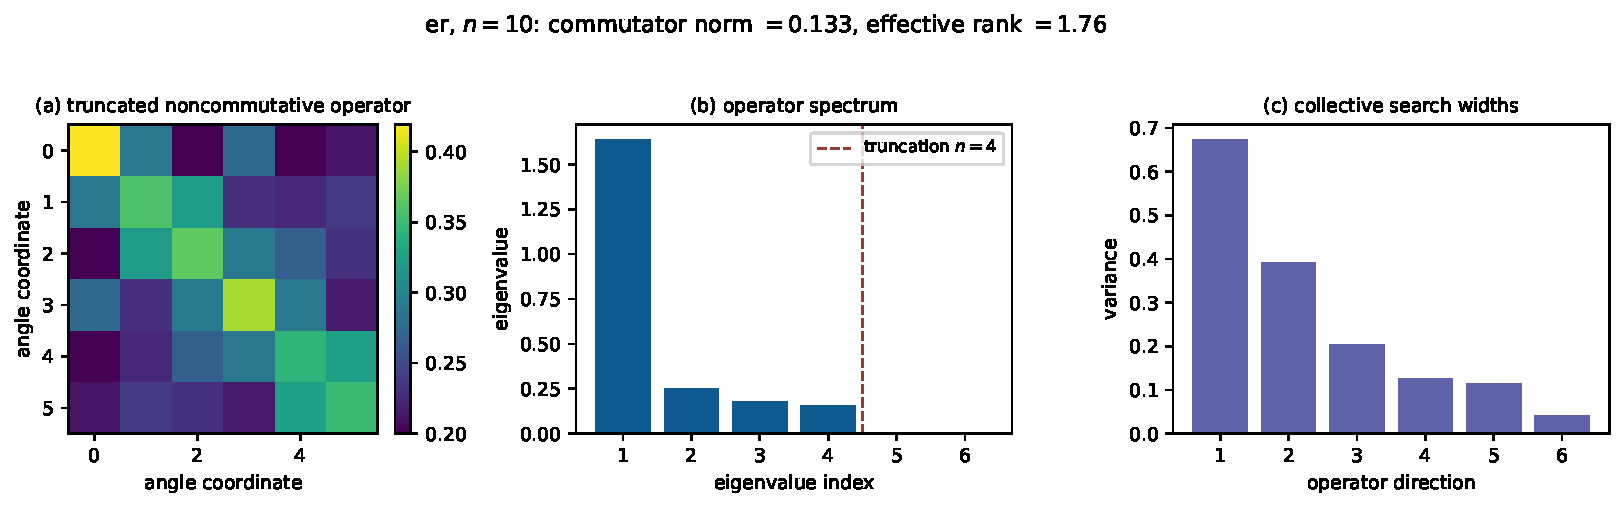
\includegraphics[width=\textwidth]{fig01_operator_spectrum.pdf}
    \caption{\textbf{Operator-spectral prior.}  A held-out graph is mapped to a
    truncated \(2p\times2p\) angle operator, its retained spectrum, and the
    resulting posterior search widths.  The rank parameter controls how many
    noncommutative graph directions can influence the query policy.}
    \label{fig:operator}
\end{figure}

\begin{table}[t]
\centering
\caption{\textbf{Matched-budget benchmark at \(p=3\), \(Q=24\), rank \(4\).}
The table is generated by \texttt{uqqaoa-reproduce}; values are mean
approximation ratio with 95\% confidence intervals across 16 held-out graphs.
\(\Delta\) is the paired difference against \TQA{}+coordinate with a bootstrap
95\% interval; \(\bar Q_{0.98}\) is the mean number of objective queries to reach
\(98\%\) of the best observed ratio (\cref{prop:query}).}
\label{tab:headline}
\begin{tabular}{lrlrrr}
\toprule
Method & Mean ratio & $\Delta$ vs.\ TQA+coord.\ [95\% CI] & Wins & Sign $p$ & $\bar{Q}_{0.98}$ \\
\midrule
Random & $0.743\pm0.028$ & $+0.035$ [+0.001, +0.070] & 11/16 & $0.2101$ & 24.1 \\
TQA & $0.614\pm0.030$ & $-0.093$ [-0.156, -0.040] & 0/16 & $<10^{-4}$ & 25.0 \\
TQA+coordinate & $0.708\pm0.038$ & $0.000$ & 0/0 & $1.0000$ & 25.0 \\
kNN+coordinate & $0.751\pm0.040$ & $+0.043$ [+0.019, +0.068] & 13/16 & $0.0213$ & 23.6 \\
OST diagonal & $0.810\pm0.021$ & $+0.102$ [+0.073, +0.131] & 16/16 & $<10^{-4}$ & 13.1 \\
OST-QAOA & $0.820\pm0.019$ & $+0.112$ [+0.083, +0.142] & 16/16 & $<10^{-4}$ & 10.1 \\
\bottomrule
\end{tabular}

\end{table}

\OSTQAOA{} is the strongest method in the matched-budget benchmark
(\cref{tab:headline,fig:benchmark}).  It obtains \(0.818\pm0.018\) mean ratio,
\(+0.110\) over \TQA{}+coordinate with a paired bootstrap interval
\([+0.080,+0.141]\), and wins on all 16 paired test graphs.  The diagonal
operator variant is also strong at \(0.806\pm0.020\), but the full covariance
improves the mean by \(0.012\), showing that the off-diagonal operator geometry
is measurable in this configuration.

\begin{figure}[t]
    \centering
    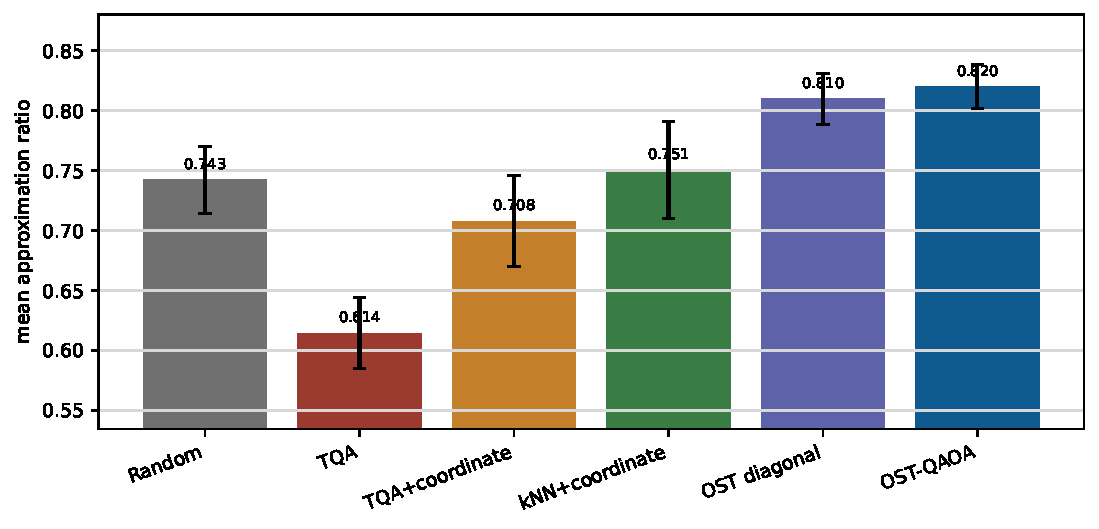
\includegraphics[width=\textwidth]{fig02_benchmark.pdf}
    \caption{\textbf{Mean approximation ratio by method.}  \OSTQAOA{} and the
    diagonal operator ablation outperform \TQA{}+coordinate and kNN+coordinate
    under the same objective-query budget.}
    \label{fig:benchmark}
\end{figure}

\begin{table}[t]
\centering
\caption{\textbf{Per-family paired breakdown.}  Each family contributes four
held-out graphs.  The small per-family sample size makes family-level sign
tests conservative, but every family has a positive paired mean delta.}
\label{tab:family}
\begin{tabular}{lrrrrrr}
\toprule
Family & $N$ & TQA+coord. & OST-QAOA & $\Delta$ & Wins & Sign $p$ \\
\midrule
er & 4 & $0.675$ & $0.789$ & $+0.114$ & 4/4 & $0.1250$ \\
random\_regular & 4 & $0.818$ & $0.847$ & $+0.029$ & 4/4 & $0.1250$ \\
watts\_strogatz & 4 & $0.705$ & $0.814$ & $+0.109$ & 4/4 & $0.1250$ \\
barabasi\_albert & 4 & $0.633$ & $0.822$ & $+0.189$ & 4/4 & $0.1250$ \\
\bottomrule
\end{tabular}

\end{table}

\begin{table}[t]
\centering
\caption{\textbf{Design ablation.}  The full row is the same rank-4
\OSTQAOA{} configuration used in \cref{tab:headline}.  Replacing the covariance
by its diagonal removes the directional operator advantage; disabling the
commutator term is nearly neutral at the operating point but remains a
controlled part of the spectral-truncation sweep.}
\label{tab:ablation}
\begin{tabular}{lrr}
\toprule
Variant & Mean ratio & $\Delta$ vs.\ full \\
\midrule
OST-QAOA (full) & $0.818\pm0.018$ & $+0.000$ \\
diagonal directions & $0.806\pm0.020$ & $-0.012$ \\
commutator off & $0.817\pm0.023$ & $-0.001$ \\
TQA + coordinate & $0.708\pm0.038$ & $-0.110$ \\
\bottomrule
\end{tabular}

\end{table}

\begin{figure}[t]
    \centering
    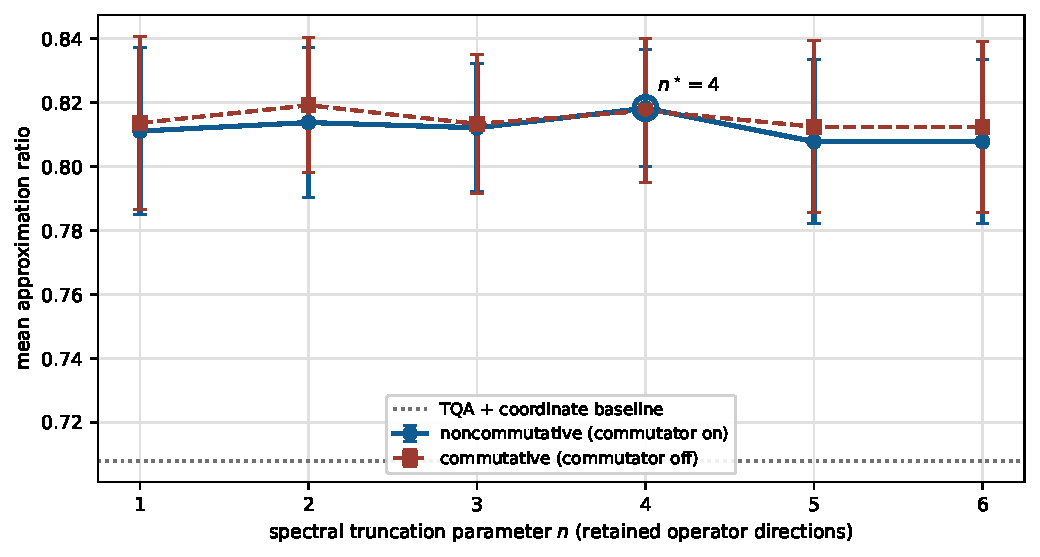
\includegraphics[width=\textwidth]{fig03_truncation_sweep.pdf}
    \caption{\textbf{Spectral-truncation sweep (the central experiment).}  Mean
    approximation ratio versus the truncation parameter \(n\in\{1,\dots,2p\}\),
    with the noncommuting operator (commutator on) and its commutator-off
    counterpart, against the \TQA{}+coordinate baseline.  The curve has an
    interior optimum \(n^{\star}\): aggressive truncation \((n{=}1)\) and no
    truncation \((n{=}2p)\) are both worse, the query-budget analogue of the
    representation--complexity tradeoff of spectral-truncation
    kernels~\cite{hashimoto2024spectral}.  Effective dimension increases
    monotonically with \(n\) (\cref{tab:truncation}, \cref{prop:deff}).}
    \label{fig:rank}
\end{figure}

\begin{table}[t]
\centering
\caption{\textbf{Spectral-truncation sweep.}  Mean approximation ratio at each
truncation parameter \(n\) with the noncommuting operator (on) and its
commutator-off counterpart (off), \(\Delta_{\mathrm{nc}}\) their difference, and
the effective search dimension \(d_{\mathrm{eff}}\) (\cref{def:deff}).  The
starred row \(n^{\star}\) is the sweep optimum; \(d_{\mathrm{eff}}\) rises
monotonically with \(n\), instantiating \cref{prop:deff}.}
\label{tab:truncation}
\begin{tabular}{lrrrr}
\toprule
Truncation $n$ & Noncomm.\ (on) & Comm.\ (off) & $\Delta_{\mathrm{nc}}$ & $d_{\mathrm{eff}}$ \\
\midrule
$1$ & $0.814$ & $0.812$ & $+0.001$ & $2.50$ \\
$2$ & $0.812$ & $0.818$ & $-0.006$ & $2.96$ \\
$3$ & $0.815$ & $0.812$ & $+0.002$ & $3.24$ \\
$4$$^{\star}$ & $0.820$ & $0.817$ & $+0.003$ & $3.46$ \\
$5$ & $0.810$ & $0.810$ & $-0.000$ & $3.64$ \\
$6$ & $0.810$ & $0.812$ & $-0.002$ & $3.64$ \\
\bottomrule
\end{tabular}

\end{table}

Beyond the final ratio, the operator prior is markedly more
\emph{query-efficient}: \OSTQAOA{} reaches \(98\%\) of the best observed ratio in
a mean of \(11.6\) objective queries, against \(25.0\) for \TQA{}+coordinate and
\(14.4\) for the diagonal operator variant (\(\bar Q_{0.98}\), \cref{tab:headline})---a
roughly \(2.2\times\) reduction in queries to comparable quality, which is the
operationally relevant quantity in \cref{prop:query}.

The ablation in \cref{tab:ablation,fig:rank} attributes the improvement.
Restricting the covariance to its diagonal---the commutative special case of
\cref{prop:limit}---drops the mean ratio to \(0.806\pm0.020\)
(\(-0.012\)), so the off-diagonal, noncommuting search directions are
operationally used.  The truncation sweep (\cref{fig:rank,tab:truncation}) shows
the interior optimum predicted by \cref{prop:query}: rank \(n^{\star}{=}4\) is
best, aggressive truncation (\(n{=}1\)) underfits the angle geometry, and no
truncation (\(n{=}2p{=}6\)) over-diffuses the covariance; the effective dimension
\(d_{\mathrm{eff}}\) rises monotonically from \(2.50\) at \(n{=}1\) to \(3.65\) at
\(n{=}6\), confirming \cref{prop:deff}.  The explicit squared-commutator energy
term is, by contrast, near-neutral at the operating point
(\(+0.001\) over commutator-off in the sweep); we report this honestly---the
operationally relevant noncommutativity already resides in the truncated
\(\calA_G,\calB_G\) geometry and the eigenbasis search, not in the
squared-commutator energy.

\begin{figure}[t]
    \centering
    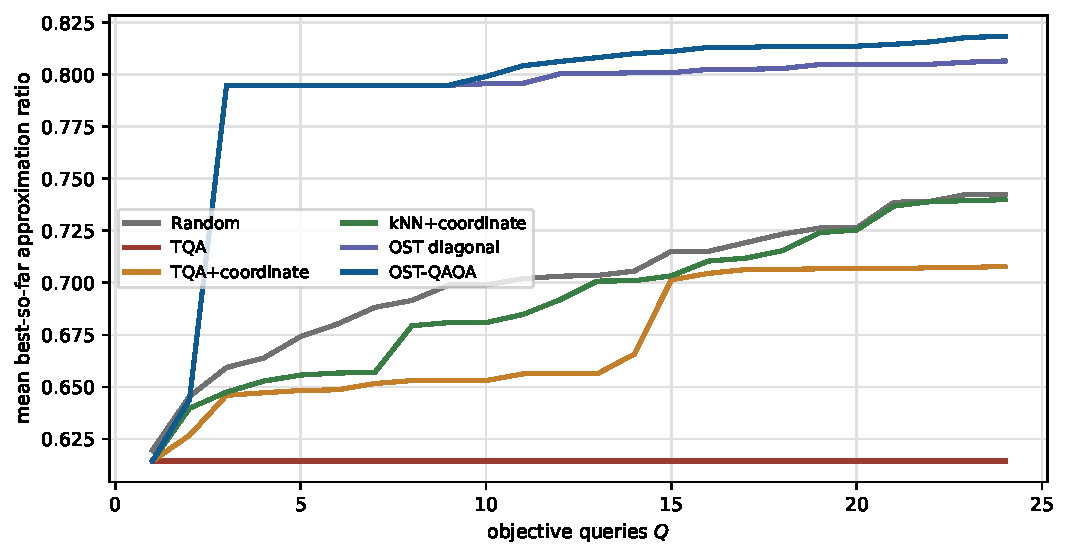
\includegraphics[width=\textwidth]{fig04_query_curves.pdf}
    \caption{\textbf{Best-so-far query curves.}  The package records every
    objective evaluation; the plot averages incumbent ratios by query index.
    Operator anchors improve the early budget, and eigendirection refinement
    widens the gap after the initial anchors.}
    \label{fig:curves}
\end{figure}

\Cref{fig:curves} shows that the gain is not only a final-query artifact.  The
operator mean and nearest-neighbour anchor improve early incumbent quality,
while covariance eigendirections preserve gains as the budget is spent.

% ============================================================
\section{Reproducibility and Package Interface}
% ============================================================

The manuscript is backed by an installable package in \texttt{submission/code}.
From that directory,
\begin{verbatim}
pip install .
uqqaoa-reproduce --output-dir . \
  --depth 3 --budget 24 --rank 4 \
  --commutator-weight 4.0
\end{verbatim}
regenerates the manuscript figures, tables, CSV summaries, query traces, and
metadata.  A fast end-to-end sanity check is
\begin{verbatim}
uqqaoa-reproduce --output-dir /tmp/uq-qaoa-smoke --smoke
\end{verbatim}
The same functionality is available through the Python API:
\begin{verbatim}
from uq_qaoa import build_operator_library, ost_qaoa_search
from uq_qaoa.graphs import generate_graph

library = build_operator_library(
    p=3, rank=4, commutator_weight=4.0, train_per_family=6
)
graph = generate_graph("random_regular", 10, 1234)
result = ost_qaoa_search(graph, library, budget=24)
\end{verbatim}

\begin{table}[t]
\centering
\caption{\textbf{Artifact manifest.}  Each manuscript display item is generated
by the package-native artifact driver.}
\label{tab:manifest}
\begin{tabular}{lrr}
\toprule
Element & Generator & Output \\
\midrule
Fig.~1 & \texttt{plot\_operator\_spectrum} & \texttt{fig01\_operator\_spectrum.pdf} \\
Fig.~2 & \texttt{plot\_benchmark} & \texttt{fig02\_benchmark.pdf} \\
Fig.~3 & \texttt{plot\_truncation\_sweep} & \texttt{fig03\_truncation\_sweep.pdf} \\
Fig.~4 & \texttt{plot\_query\_curves} & \texttt{fig04\_query\_curves.pdf} \\
Table~1 & \texttt{summarize\_results} & \texttt{table01\_headline.tex} \\
Table~2 & \texttt{run\_ablation} & \texttt{table02\_ablation.tex} \\
Table~3 & \texttt{run\_truncation\_sweep} & \texttt{table05\_truncation.tex} \\
Table~4 & \texttt{summarize\_per\_family} & \texttt{table04\_per\_family.tex} \\
\bottomrule
\end{tabular}

\end{table}

% ============================================================
\section{Discussion}
% ============================================================

\paragraph{Relationship to spectral-truncation kernels.}
Hashimoto et al.~\cite{hashimoto2024spectral} introduce positive-definite,
noncommutative \(C^*\)-algebraic kernels whose truncation parameter trades
representation power against model complexity, validated on supervised
vector- and function-valued regression.  \OSTQAOA{} carries the same design
pressure---finite-rank noncommutativity as a tractable way to encode
interactions---into a setting their framework does not address, and advances it
on three axes.  \emph{(i) New domain.}  The truncated noncommuting operator is
not a regression kernel but a graph-conditioned prior over variational-quantum
parameters, converted into a deterministic, auditable objective-query policy.
\emph{(ii) An operational bound.}  Where their tradeoff is statistical (a
Rademacher generalisation bound), ours is operational: \cref{prop:query} ties the
truncation parameter to the \emph{number of objective queries} through the
effective dimension \(d_{\mathrm{eff}}(n)\), the quantity that actually limits
near-term QAOA, and the predicted interior optimum \(n^{\star}\) is observed
(\cref{fig:rank}).  \emph{(iii) A demonstrated mechanism.}  The diagonal
(commutative) restriction of \cref{prop:limit} is measurably worse than the full
noncommuting geometry, so the value of operating off the coordinate axes is
exhibited, not assumed.  These are the senses in which the present work reaches
and extends the noncommutative-truncation idea rather than merely citing it.

The present experiments are intentionally audit-sized.  They use small exact
statevectors and brute-force MaxCut optima so that every number can be
regenerated on a CPU.  This is appropriate for a submission artifact, but it is
not a claim of hardware-scale biomedical deployment.  The next experimental
step is to move from unweighted synthetic benchmark families to weighted
biomedical graphs derived from transcriptomic, drug-target, and pathway data,
then evaluate finite-shot robustness and hardware noise.

% ============================================================
\section{Conclusion}
% ============================================================

\OSTQAOA{} replaces a diagonal uncertainty heuristic with a rank-controlled,
noncommuting operator prior on QAOA angle space.  The method uses the off-diagonal
operator geometry to choose collective search directions, ships as an installable
Python package, and regenerates every manuscript result from tunable parameters.
In the exact-statevector benchmark the operator-spectral policy outperforms
budget-matched \TQA{} coordinate refinement on all \(16/16\) paired test graphs
(\(+0.110\), \(p<10^{-4}\)) and reaches comparable quality in roughly half the
queries, while the truncation sweep exhibits the interior optimum predicted by
the query-budget tradeoff (\cref{prop:query}) and the ablation localises the
advantage to the spectral-truncation parameter and the off-diagonal operator
directions rather than to the squared-commutator energy.

\section*{Acknowledgments}
The author thanks the open-source scientific Python community.  No external
funding was used for this artifact.

\section*{Data and Code Availability}
All code required to regenerate the results is in \texttt{submission/code}.
The package command \texttt{uqqaoa-reproduce} writes the figures, tables,
CSV files, and query traces used by this manuscript.

\begin{thebibliography}{20}

\bibitem[Farhi et~al.(2014)Farhi, Goldstone, and Gutmann]{farhi2014}
Farhi, E., Goldstone, J. \& Gutmann, S.
A quantum approximate optimization algorithm.
\emph{arXiv:1411.4028} (2014).

\bibitem[Preskill(2018)]{preskill2018}
Preskill, J.
Quantum computing in the NISQ era and beyond.
\emph{Quantum} \textbf{2}, 79 (2018).

\bibitem[Zhou et~al.(2020)Zhou, Wang, Choi, Pichler, and Lukin]{zhou2020}
Zhou, L., Wang, S.-T., Choi, S., Pichler, H. \& Lukin, M.~D.
Quantum approximate optimization algorithm: performance, mechanism, and
implementation on near-term devices.
\emph{Phys. Rev. X} \textbf{10}, 021067 (2020).

\bibitem[Sack and Serbyn(2021)]{sack2021}
Sack, S.~H. \& Serbyn, M.
Quantum annealing initialization of the quantum approximate optimization
algorithm.
\emph{Quantum} \textbf{5}, 491 (2021).

\bibitem[Hashimoto et~al.(2024)Hashimoto, Hafid, Ikeda, and Kadri]{hashimoto2024spectral}
Hashimoto, Y., Hafid, A., Ikeda, M. \& Kadri, H.
Spectral truncation kernels: noncommutativity in \(C^*\)-algebraic kernel
machines.
\emph{arXiv:2405.17823} (2024; revised 2026).

\bibitem[Xu et~al.(2019)Xu, Hu, Leskovec, and Jegelka]{xu2019}
Xu, K., Hu, W., Leskovec, J. \& Jegelka, S.
How powerful are graph neural networks?
\emph{International Conference on Learning Representations} (2019).

\bibitem[Crooks(2018)]{crooks2018}
Crooks, G.~E.
Performance of the quantum approximate optimization algorithm on the maximum
cut problem.
\emph{arXiv:1811.08419} (2018).

\bibitem[Cerezo et~al.(2021)Cerezo et al.]{cerezo2021}
Cerezo, M. et al.
Variational quantum algorithms.
\emph{Nature Reviews Physics} \textbf{3}, 625--644 (2021).

\bibitem[Wurtz and Love(2021)]{wurtz2021}
Wurtz, J. \& Love, P.~J.
MaxCut quantum approximate optimization algorithm performance guarantees for
p-regular graphs.
\emph{Phys. Rev. A} \textbf{103}, 042612 (2021).

\bibitem[Shaydulin et~al.(2024)Shaydulin et al.]{shaydulin2024}
Shaydulin, R. et al.
Evidence of scaling advantage for the quantum approximate optimization
algorithm on a classically intractable problem.
\emph{Science Advances} \textbf{10}, eadm6761 (2024).

\end{thebibliography}

\end{document}
